\documentclass{article}
\usepackage{graphicx} % Required for inserting images
\usepackage{float}  % Import the float package to use [H] specifier
\usepackage{booktabs}

\setcounter{secnumdepth}{4}

\title{Labwork 10: Gather and Scatter\\Fine-art Transformation}
\author{Pham Gia Phuc}
\date{November 2024}

\begin{document}

\maketitle

\setlength\parindent{0pt}

\section{Subject}
This lab aims to implement the Kuwahara filter in CUDA, both with and without shared memory.

\section{Implementation}

    \subsection{Preparation}
    This report uses a CUDA kernel provided by Google Colaboratory.

    \begin{table}[ht]
        \centering
        \begin{tabular}{@{}ll@{}}
            \textbf{Attribute} & \textbf{Value} \\
            Number of CUDA Devices Found & 1 \\
            Device ID & 0 \\
            Name & Tesla T4 \\
            Compute Capability & 7.5 \\
            PCI Device ID & 4 \\
            PCI Bus ID & 0 \\
            UUID & GPU-af936f72-170a-716a-326e-6053e93d8f54 \\
            Watchdog & Disabled \\
            FP32/FP64 Performance Ratio & 32 \\
            Multiprocessor Count & 40 \\
            Approximate Core Count & 2560 \\
            Total Memory Size & 14.75 GB \\
            Environment & Google Colab \\ 
        \end{tabular}
        \caption{CUDA Device Information}
        \label{tab:cuda_device_info}
    \end{table}

    \subsection{Kuwahara Kernel}
    The Kuwahara filter is a non-linear smoothing filter used in image processing for adaptive noise reduction. Unlike typical linear low-pass filters, which reduce noise but blur edges, the Kuwahara filter smooths an image while preserving edges. It divides a window into four square regions (a, b, c, and d), as illustrated in Figure~\ref{fig:kuwahara-window}, with overlapping central rows and columns.

    \begin{figure}
        \centering
        \includegraphics[width=0.2\linewidth]{Kuwahara.jpg}
        \caption{Window used by a Kuwahara filter. It is divided into 4 square regions: a, b, c, and d. Pixels in the central row and column belong to multiple regions.}
        \label{fig:kuwahara-window}
    \end{figure}

    The Kuwahara filter serves the following purposes:
    \begin{itemize}
        \item Noise reduction
        \item Edge preservation
        \item Creation of an "oil painting" effect
    \end{itemize}

\section{Results}

    \subsection{Sample Image and Filter Application}
    A sample image, as shown in Figure~\ref{fig:sample-image}, was processed using the Kuwahara filter kernel to achieve an oil painting effect.

    \begin{figure}[H]
        \centering
        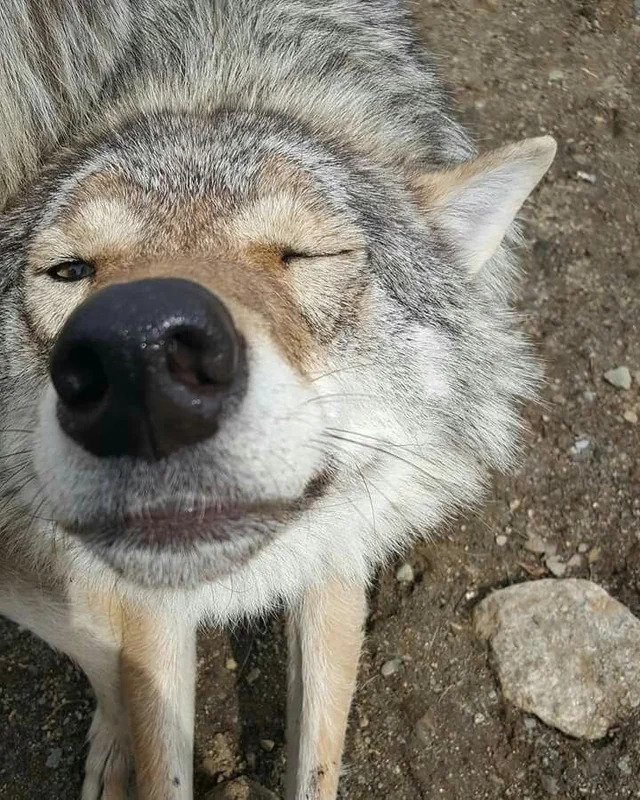
\includegraphics[width=0.3\linewidth]{wolf.jpg}
        \caption{A sample image}
        \label{fig:sample-image}
    \end{figure}

    % The filter was applied to various image resolutions, yielding the results in Figures~\ref{fig:sample_result_small} and \ref{fig:sample_result_big}. These images illustrate the filter's effectiveness in producing an oil effect while preserving edges.

    % \begin{figure}
    %     \centering
    %     \includegraphics[width=0.3\linewidth]{rsmall.png}
    %     \caption{Filtered result with a 640x800 pixel image}
    %     \label{fig:sample_result_small}
    % \end{figure}
    
    % \begin{figure}
    %     \centering
    %     \includegraphics[width=0.3\linewidth]{rbig.png}
    %     \caption{Filtered result with a 9000x5625 pixel image}
    %     \label{fig:sample_result_big}
    % \end{figure}

    The filter was applied to various image resolutions, yielding the results in Figures~\ref{fig:sample_results}. These images illustrate the filter's effectiveness in producing an oil effect while preserving edges.
    
    \begin{figure}[H]
        \centering
        \includegraphics[height=0.4\linewidth]{rsmall.png}
        \includegraphics[height=0.4\linewidth]{rbig.png}
        \caption{Filtered results with the Kuwahara filter.}
        \label{fig:sample_results}
    \end{figure}

    \subsection{Performance Analysis}
    The performance of the Kuwahara kernel was analyzed on images of different resolutions to understand the effect of using shared memory in a CUDA environment.

    For a lower-resolution image (640x800), using shared memory resulted in a marginally higher runtime compared to not using it, as shown in Table~\ref{tab:result_shared_memory_small}.

    \begin{table}[H]
        \centering
        \begin{tabular}{ccc}
           \textbf{Using Shared Memory} & \textbf{Resolution} & \textbf{Time (seconds)} \\
           Yes & 640x800 & 0.05 \\
           No  & 640x800 & 0.04 \\
        \end{tabular}
        \caption{Runtime comparison on a 640x800 image}
        \label{tab:result_shared_memory_small}
    \end{table}

    For a higher-resolution image (9000x5625), shared memory usage reduced runtime slightly, as shown in Table~\ref{tab:result_shared_memory_big}.

    \begin{table}[H]
        \centering
        \begin{tabular}{ccc}
           \textbf{Using Shared Memory} & \textbf{Resolution} & \textbf{Time (seconds)} \\
           Yes & 9000x5625 & 2.46 \\
           No  & 9000x5625 & 2.48 \\
        \end{tabular}
        \caption{Runtime comparison on a 9000x5625 image}
        \label{tab:result_shared_memory_big}
    \end{table}

\section{Conclusion}
    Using shared memory in CUDA can boost program performance, particularly with large images that require significant computation. However, for smaller images, the overhead from shared memory management can outweigh its benefits. Consequently, it is most effective to bypass shared memory for small images while leveraging it for larger images to enhance performance in Kuwahara filter applications.

\end{document}
